\documentclass[a4paper, 12pt]{article}
\usepackage[utf8]{inputenc}
\usepackage{polski}
\usepackage{hyperref}
\usepackage{graphicx}
\usepackage{indentfirst}
\usepackage{float}
\usepackage{amsfonts}

\title{Metody odkrywania wiedzy -- wykrywanie ataków sieciowych}
\author{Adam Stelmaszczyk\\ Anna Stępień}

\begin{document}
\bibliographystyle{unsrt}
\nocite{*}
\maketitle

\tableofcontents

\newpage

\section{Interpretacja tematu projektu}
Projekt ma na celu analizę działania różnych algorytmów klasyfikacji zastosowanych
w procesie wykrywania ataków sieciowych. Połączenia sieciowe można zaklasyfikować do jednej
z pięciu klas:
\begin{itemize}
  \item normal -- połączenia prawidłowe,
  \item probe -- odpytywanie, np. skanowanie portów,
  \item dos -- ataki typu Denial of Service,
  \item u2r -- ataki typu User to Root, polegające na przejęciu praw administratora, 
np. ataki przepełnienia bufora,
  \item r2l -- ataki typu Remote to Local, polegające na nieautoryzowanym dostępie ze zdalnego komputera.
\end{itemize} 

\section{Opis wykorzystanych algorytmów}\label{algorithms}

\subsection{k-NN}

k-NN jest algorytmem, który dokonuje klasyfikacji na podstawie podobieństwa do k 
najbardziej podobnych przykładów ze zbioru uczącego. W~celu oszacowania podobieństwa 
poszczególnych próbek, stosowane są miary odległości takie jak np. metryka euklidesowa lub Manhattan. 
Klasa, która przypisywana jest do badanego obiektu ustalana jest na podstawie klasy 
reprezentowanej przez największą spośród wybranych wcześniej k przykładów.

Algorytm k-NN zostanie przetestowany z~wykorzystaniem funkcji 
\texttt{knn} oferowanej przez pakiet \texttt{FNN} języka~R 
\footnote{\url{http://cran.r-project.org/web/packages/FNN/}}.

\subsection{Naiwny klasyfikator Bayesa}

Klasyfikator Bayesa wybiera klasę, która jest najbardziej prawdopodobna dla danego przykładu na 
podstawie prawdopodobieństwa
warunkowego $P(c \mid x)$, gdzie $c$ oznacza etykietę klasy, a $x$ jest przykładem. 
Jest to tzw. prawdopodobieństwo
\textit{a posteriori}. Wyznaczane jest ze wzoru:

$$ P(c \mid x) = \frac{P(x \mid c)P(c)}{P(x)} $$

Przy poszukiwaniu maksimum $P(c \mid x)$ mianownik $P(x)$ można pominąć bez zmiany wyniku 
maksymalizacji.
Prawdopodobieństwo \textit{a posteriori} $P(c)$ można oszacować na podstawie częstości 
występowania klas w zbiorze treningowym.
Natomiast prawdopodobieństwo $P(x \mid c)$ jest szacowane ze wzoru:

$$ P(x \mid c) = \prod_{i=1}^n P(a_i(x) \mid c)$$

gdzie $a_i(x)$ oznacza $i$-ty atrybut przykładu $x$.
Przyjęte zostało założenie, że wartości poszczególnych atrybutów są niezależne od siebie.
Na tym polega ,,naiwność'' klasyfikatora Bayesa.

Naiwny klasyfikator Bayesa zostanie przetestowany przy pomocy funkcji \texttt{naiveBayes} z~pakietu \texttt{e1071} języka~R
\footnote{\url{http://www-users.cs.york.ac.uk/~jc/teaching/arin/R_practical/}}.

\subsection{SVM}
SVM jest klasyfikatorem binarnym, który ma na celu wyznaczenie hiperpłaszczyzny rozdzielającej 
z~maksymalnym marginesem przykłady należące do dwóch klas. W~ramach projektu realizowana będzie 
klasyfikacja mająca na celu przypisanie połączeń sieciowych do jednej z~pięciu klas. 
Problem klasyfikacji wieloklasowej może być zdekomponowany do szeregu problemów klasyfikacji binarnej. 
W~projekcie wykorzystane zostanie podejście \textit{one-against-one}, 
które polega na zbudowaniu klasyfikatora SVM dla każdej pary klas. 

Do przetestowania klasyfikatora SVM zostanie wykorzystana funkcja \texttt{svm} z~pakietu 
\texttt{e1071} języka~R \footnote{\url{http://cran.r-project.org/web/packages/e1071/}}.

\section{Przygotowanie danych}

Podczas realizacji projektu został wykorzystany zbiór danych z konkursu 
KDD'99 Classifier Learning Contest
\footnote{\url{www.sigkdd.org/kdd-cup-1999-computer-network-intrusion-detection}}.
Każdy przykład zawiera 41 atrybutów połączenia sieciowego. W poniższej tabeli przedstawiono
szczegóły wszystkich atrybutów.
42 kolumna danych treningowych zawiera typ ataku, który bezpośrednio mapuje się na
jedną z pięciu ostatecznych klas. \\

\begin{tabular}{ | l | p{3cm} | p{3cm} | p{6cm} | } \hline
Nr & Nazwa & Opis & Zbiór wartości \\ \hline
1*      & duration & czas połączenia w sekundach & $\mathbb Z_{\ge 0}$ \\ \hline
2*      & protocol\_type & rodzaj protokołu & icmp, tcp, udp \\ \hline
3*      & service & usługa na serwerze & smtp, bgp, imap4, courier, name, exec, ftp, echo, http\_2784,
                       http\_443, discard, kshell, login, http, Z39\_50, vmnet, supdup,
                       gopher, printer, aol, tftp\_u, csnet\_ns, http\_8001, eco\_i, time,
                       ssh, efs, hostnames, X11, klogin, sql\_net, ldap, private,
                       auth, uucp, pm\_dump, link, ctf, IRC, ecr\_i, netbios\_ns, urp\_i,
                       pop\_2, pop\_3, rje, systat, ftp\_data,finger, tim\_i, remote\_job,
                       other, domain\_u, urh\_i, iso\_tsap, netstat, daytime, whois, shell,
                       mtp, sunrpc, uucp\_path, red\_i, harvest, nnsp, telnet, domain,
                       ntp\_u, netbios\_dgm, nntp, netbios\_ssn \\ \hline
4      & flag & status połączenia & REJ, SF, SH, RSTO, OTH, RSTR, RSTOS0, S0, S1, S2, S3 \\ \hline
5*      & src\_bytes  & bajty przesłane w połączeniu & $\mathbb Z_{\ge 0}$ \\ \hline
6*      & dst\_bytes  & bajty pobrane w połączeniu  & $\mathbb Z_{\ge 0}$ \\ \hline
7      & land & 1, jeśli źródło oraz cel połączenia ma tego samego hosta i port & 0, 1 \\ \hline
8      & wrong\_fragment  & liczba pakietów oznaczonych jako ,,wrong'' & $\mathbb Z_{\ge 0}$ \\ \hline
9      & urgent  & liczba pakietów oznaczonych jako ,,urgent''  & $\mathbb Z_{\ge 0}$ \\ \hline
\end{tabular}

\begin{tabular}{ | l | l | p{6cm} | p{2,1cm} | } \hline
Nr & Nazwa & Opis & Zbiór wartości \\ \hline
10      & hot & liczba wskaźników ,,hot'' dla akcji, np. uruchamianie programów & $\mathbb Z_{\ge 0}$ \\ \hline
11      & num\_failed\_logins  & liczba nieudanych prób logowania w połączeniu & $\mathbb Z_{\ge 0}$ \\ \hline
12*      & logged\_in  & 1, jeśli udało się zalogować &  0, 1 \\ \hline
13      & num\_compromised & liczba wystąpień błędu ,,not found'' podczas połączenia &  $\mathbb Z_{\ge 0}$ \\ \hline
14      & root\_shell  & 1, jeśli uzyskano konsolę z uprawnieniami root  &  0, 1 \\ \hline
15      & su\_attempted  & 1, jeśli użyto komendy \texttt{su} &  0, 1 \\ \hline
16      & num\_root  & liczba operacji wykonanych jako root  & $\mathbb Z_{\ge 0}$ \\ \hline
17      & num\_file\_creations  & liczba utworzonych plików  & $\mathbb Z_{\ge 0}$ \\ \hline
18      & num\_shells  & liczba zalogowań jako normalny użytkownik & $\mathbb Z_{\ge 0}$ \\ \hline
19      & num\_access\_files  & liczba operacji na plikach kontroli dostępu & $\mathbb Z_{\ge 0}$ \\ \hline
20      & num\_outbound\_cmds & liczba poleceń wychodzących w sesji FTP & $\mathbb Z_{\ge 0}$ \\ \hline
21      & is\_hot\_login  & 1, jeśli login należy to listy ,,hot'', tzn. jeśli login to root albo adm &  0, 1 \\ \hline
22      & is\_guest\_login  & 1, jeśli login należy to listy ,,guest'' &  0, 1 \\ \hline
23*     & count & liczba połączeń do tego samego hosta w przeciągu 2 sekund & $\mathbb Z_{\ge 0}$ \\ \hline
24*      & srv\_count   & liczba połączeń z tą samą usługą w przeciągu 2 sekund &  $\mathbb Z_{\ge 0}$ \\ \hline
25      & serror\_rate        & \% połączeń o tym samym hoście z błędami SYN  & $\mathbb{R} \in [0; 1]$ \\ \hline
26      & srv\_serror\_rate   & \% połączeń do tej samej usługi z błędami SYN & $\mathbb{R} \in [0; 1]$ \\ \hline
27      & rerror\_rate        & \% połączeń o tym samym hoście z błędami REJ   & $\mathbb{R} \in [0; 1]$ \\ \hline
28      & srv\_rerror\_rate   & \% połączeń do tej samej usługi z błędami REJ  & $\mathbb{R} \in [0; 1]$ \\ \hline
29*      & same\_srv\_rate     & \% połączeń do tej samej usługi  &  $\mathbb{R} \in [0; 1]$ \\ \hline
30      & diff\_srv\_rate     & \% połączeń do różnych usług &  $\mathbb{R} \in [0; 1]$ \\ \hline  
31*      & srv\_diff\_host\_rate   & \% połączeń do różnych hostów   & $\mathbb{R} \in [0; 1]$ \\ \hline
\end{tabular}

\begin{tabular}{ | l | l | p{5cm} | p{1,9cm} | } \hline
Nr & Nazwa & Opis & Zbiór wartości \\ \hline
32      & dst\_host\_count & liczba połączeń do tego samego adresu IP  &  $\mathbb Z_{\ge 0}$ \\ \hline
33      & dst\_host\_srv\_count  & liczba połączeń do tego samego portu docelowego   & $\mathbb Z_{\ge 0}$ \\ \hline
34      & dst\_host\_same\_srv\_rate  & \% połączeń do tej samej usługi w stosunku do liczby połączeń do tego samego adresu IP (atrybut 31) & $\mathbb{R} \in [0; 1]$ \\ \hline
35*      & dst\_host\_diff\_srv\_rate  & \% połączeń do tej różnych usług w stosunku do liczby połączeń do tego samego adresu IP (atrybut 31) & $\mathbb{R} \in [0; 1]$ \\ \hline
36*      & dst\_host\_same\_src\_port\_rate & \% połączeń do tego samego portu źródłowego w stosunku do liczby połączeń do tego samego portu docelowego (atrybut 32)  & $\mathbb{R} \in [0; 1]$ \\ \hline
37*      & dst\_host\_srv\_diff\_host\_rate & \% połączeń do różnych portów źródłowych w stosunku do liczby połączeń do tego samego portu docelowego (atrybut 32)  &  $\mathbb{R} \in [0; 1]$ \\ \hline

38*      & dst\_host\_serror\_rate       & \% połączeń o tym samym hoście z błędami SYN w stosunku do atrybutu 31        &  $\mathbb{R} \in [0; 1]$ \\ \hline  
39      & dst\_host\_srv\_serror\_rate  & \% połączeń o tym samym hoście z błędami SYN w stosunku do atrybutu 32 & $\mathbb{R} \in [0; 1]$ \\ \hline

40      & dst\_host\_rerror\_rate        & \% połączeń o tym samym hoście z błędami REJ w stosunku do atrybutu 31 & $\mathbb{R} \in [0; 1]$ \\ \hline
41      & dst\_host\_srv\_rerror\_rate   & \% połączeń o tym samym hoście z błędami REJ w stosunku do atrybutu 32 & $\mathbb{R} \in [0; 1]$ \\ \hline
\end{tabular}

\begin{tabular}{ | l | l | p{4,5cm} | p{5,3cm} | } \hline
Nr & Nazwa & Opis & Zbiór wartości \\ \hline
42      & attack\_type & rodzaj ataku sieciowego & back, buffer\_overflow, ftp\_write, guess\_passwd, imap, ipsweep, land, loadmodule, multihop, neptune, nmap, normal, perl, phf, pod, portsweep, rootkit, satan, smurf, spy, teardrop, warezclient, warezmaster \\ \hline
\end{tabular} \\\\

Znakiem gwiazdki (*) oznaczono 14 atrybutów wybranych do klasyfikacji.
Sposób w jaki je wybrano opisano w rozdziale \ref{sec:selekcja}.

\section{Statystyczny opis danych}

Podczas testów wykorzystane zostały dwa zbiory treningowe -- pełny zbiór treningowy 
liczący 4898431 przykładów oraz jego losowy, 1-procentowy podzbiór.
W~tabeli \ref{table:100percent} został przedstawiony rozkład klas przykładów w~pełnym zbiorze
treningowym. 

\begin{table}[H]
\centering
\begin{tabular}{ | l | l | l | l | l | l | } \hline
	normal & probe & dos & u2r & r2l & razem \\  \hline
	972780 & 41102 & 3883370 & 52 & 1126 & 4898431 \\ \hline
	19.86\% & 0.84\% & 79.28\% & 0.001\% & 0.023\% & \\ \hline
\end{tabular}
\caption{Rozkład klas w pełnym zbiorze treningowym.}
\label{table:100percent}
\end{table}

W~tabeli \ref{table:1percent} został przedstawiony rozkład klas przykładów w 
zbiorze treningowym będącym losowym, 1-procentowym
podzbiorem pełnego zbioru treningowego.
\begin{table}[H]
\centering
\begin{tabular}{ | l | l | l | l | l | l | } \hline
	normal & probe & dos & u2r & r2l & razem \\ \hline
	9725 & 414 & 38831 & 2 & 12 & 48984 \\ \hline
	19.85\%  & 0.85\%  & 79.27\% & 0.004\%  & 0.024\% &  \\ \hline
\end{tabular}
\caption{Rozkład klas w zbiorze treningowym będącym losowym, 1-procentowym
 podzbiorem pełnego zbioru treningowego.}
\label{table:1percent}
\end{table}

W~tabeli \ref{table:test} został przedstawiony rozkład klas przykładów w zbiorze testowym.
\begin{table}[H]
\centering
	\begin{tabular}{ | l | l | l | l | l | l | } \hline
		normal & probe & dos & u2r & r2l & razem \\ \hline
		60592 & 4166 & 229853 & 228 & 16189 & 311028 \\ \hline
		19.48\% & 1.34\% & 73.9\% & 0.073\%  & 5.2\% & \\ \hline
	\end{tabular}
\caption{Rozkład klas w zbiorze testowym.}
\label{table:test}
\end{table}

Konkursowy zbiór testowy posiadał zupełnie inny empiryczny rozkład prawdopodobieństwa klas niż zbiór treningowy.
Największa różnica liczby przykładów wystąpiła dla klasy r2l. Zbiór trenujący posiada zaledwie
1126 przykładów tej klasy (0,023\% całości), natomiast zbiór testujący aż 16189 (5,2\% całego
zbioru testującego). Zbiór testujący posiada około 14 razy więcej przykładów r2l niż zbiór
trenujący, pomimo tego, że jest około 16 razy mniejszy od niego. Powoduje to, że klasa r2l
jest najtrudniej rozpoznawalna, co potwierdzają wyniki przedstawione w rozdziale \ref{sec:wyniki}.

\section{Transformacja danych}

Na początku dane zostały przejrzane w poszukiwaniu pojedynczych wartości odstających
powstałych np. na skutek błędu ludzkiego. Dokonano tego przy pomocy funkcji \texttt{summary}
języka R. Nie znaleziono wartości odstających.

Po wczytaniu danych z pliku tekstowego przeprowadzane zostały następujące kroki:
\begin{enumerate}
 \item Dla SVM, zbiór wejściowy jest zmniejszany do 1\%.
 \item Atrybuty wyliczeniowe są zamieniane na liczbowe.
 \item Wybieranych jest 14 atrybutów.
 \item Wartości w kolumnach są normalizowane, by miały średnią równą 0 i~standardowe odchylenie równe 1.
\end{enumerate}
Tak przetworzony zbiór trenujący i testowy został zapisany do skompresowanego pliku \texttt{.processed}.
Plik ten może być szybko wczytywany przez testowane algorytmy, bez potrzeby
transformowania danych za każdym razem.

Wykorzystywane w~projekcie dane charakteryzują się nierównomiernym rozkładem klas. 
Dlatego przetestowano resampling przykładów treningowych, w~celu uzyskania równomiernego rozkładu klas. 
Wykorzystany został algorytm \texttt{SMOTE} udostępniany przez pakiet 
\texttt{DMwR} \footnote{\url{http://cran.r-project.org/web/packages/DMwR/}} języka~R.
Wyniki przedstawiono w rozdziale \ref{smote}.

\section{Selekcja atrybutów}
\label{sec:selekcja}

Wykorzystana została funkcja \texttt{importance} z pakietu lasów losowych
\footnote{\url{http://cran.r-project.org/web/packages/randomForest/randomForest.pdf}}.
Wynik jej wywołania dla pełnego zbioru trenującego przedstawiono na rysunku \ref{fig:attr}.

\begin{figure}[H]
\centering
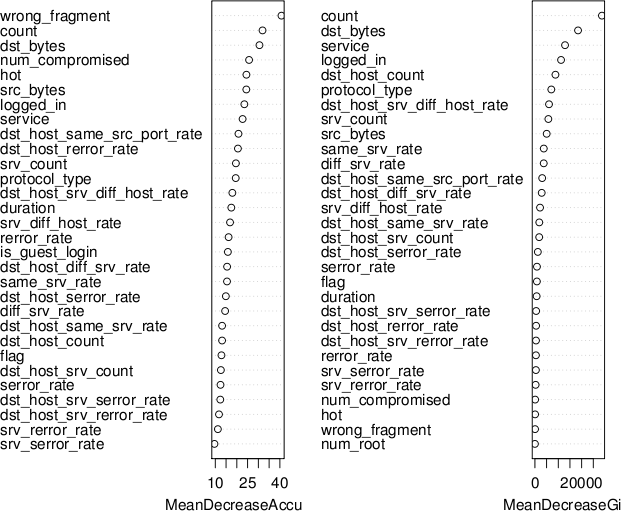
\includegraphics[width=.9\textwidth]{attr}
\caption{Wynik wywołania \texttt{importance} przedstawia 30 ,,najważniejszych'' atrybutów
dla dwóch miar. 
Po lewej stronie miara średniego spadku precyzji.
Po prawej stronie miara średniego spadku indeksu Giniego. 
Im atrybut wyżej się znajduje, tym ,,ważniejszy''.}
\label{fig:attr}
\end{figure}

Rozmiar przecięcia zbioru atrybutów wskazanych przez spadek precyzji ze zbiorem
atrybutów wskazanych przez indeks Giniego wynosi 29. Uznano, że 29 jest jeszcze zbyt dużą liczbą
wymiarów, dlatego przygotowano rankingi 20 ,,najważniejszych'' atrybutów, nie 30.
Rozmiar przecięcia takich zbiorów wyniósł 14 i te atrybuty zdecydowano się wykorzystać 
w klasyfikacji: 
\begin{itemize}
	\item duration, protocol\_type,
	\item service, src\_bytes,
	\item dst\_bytes,
	\item logged\_in,
	\item count, srv\_count,
	\item same\_srv\_rate, 
	\item srv\_diff\_host\_rate, 
	\item dst\_host\_diff\_srv\_rate, 
	\item dst\_host\_same\_src\_port\_rate,
	\item dst\_host\_diff\_src\_port\_rate, 
	\item dst\_host\_serror\_rate.
\end{itemize}
Na końcu rankingów zwróconych przez \texttt{importance} znalazły się atrybuty:
\begin{itemize}
	\item num\_failed\_logins,
	\item root\_shell,
	\item num\_outbound\_cmds,
	\item is\_host\_login,
	\item urgent.
\end{itemize}   

\section{Ocena jakości modeli}

Do porównywania jakości modeli wykorzystano błąd klasyfikacji na zbiorze testowym 
\texttt{corrected}\footnote{\url{http://www-cse.ucsd.edu/users/elkan/corrected.gz}},
przygotowanym przez autorów konkursu KDD'99.
Zbiór ten zawiera 311028 przykładów. 
Uczestnicy KDD'99 do oceny swoich rozwiązań używali tego samego zbioru testowego,
co umożliwia porównanie wyników otrzymanych w tej pracy z wynikami z konkursu.

\section{Wyniki eksperymentów oraz wnioski}
\label{sec:wyniki}

W tym rozdziale przedstawiono wyniki eksperymentów dla trzech wybranych algorytmów:
k-NN, naiwnego Bayesa oraz SVM. 
Rozwiązaniem referencyjnym będzie rozwiązanie zwycięzcy konkursu KDD'99,
o łącznym błędzie klasyfikacji równym 7.29\%. Macierz pomyłek dla 
tego rozwiązania wygląda następująco:

\begin{table}[H]
\centering
\begin{tabular}{ | l | l | l | l | l | l | l | } \hline
	& normal & probe & dos 	& u2r 	& r2l 	& Poprawnych	\\ \hline
normal 	& 60262 & 243 	& 78	& 4	& 6 	& 99.5\% 	\\ \hline
probe 	& 511 	& 3471 	& 184	& 0	& 0 	& 83.3\% 	\\ \hline
dos 	& 5299 	& 1328 	& 223226& 0 	& 0 	& 97.1\% 	\\ \hline
u2r 	& 168 	& 20 	& 0	& 30	& 10	& 13.2\%	\\ \hline
r2l 	& 14527 & 294 	& 0	& 8	& 1360	& 8.4\%		\\ \hline
\end{tabular} 
\end{table}

Wartość 14527 oznacza, że 14527 przykładów, które faktycznie należały do klasy r2l, zaklasyfikowano
jako normal.

\subsection{k-NN}

Algorytm k-NN w wersji kd-tree został wielokrotnie uruchomiony na pełnym zbiorze trenującym
z różnymi wartościami $k$.
Dla $k=3$ osiągnięto najniższy błąd klasyfikacji na zbiorze testowym równy 7.68\%:

\begin{table}[H]
\centering
\begin{tabular}{ | r | r | r | } \hline
$k$ & Błąd klasyfikacji & Czas w sekundach \\ \hline
1 & 7.76\% & 695 \\ \hline
3 & 7.68\% & 691 \\ \hline
5 & 7.75\% & 706 \\ \hline
7 & 7.76\% & 615 \\ \hline
9 & 7.77\% & 716 \\ \hline
\end{tabular} 
\end{table}

Czas wykonywania algorytmu wynosił od 10 do 12 minut.
Macierz pomyłek dla najlepszego wariantu 3-NN wyglądała następująco:

\begin{table}[H]
\centering
\begin{tabular}{ | l | l | l | l | l | l | l | } \hline
	& normal & probe & dos 	& u2r 	& r2l 	& Poprawnych	\\ \hline
normal 	& 59953 & 518 	& 118	& 0	& 3 	& 98.9\% 	\\ \hline
probe 	& 255 	& 3446 	& 465	& 0	& 0 	& 82.7\% 	\\ \hline
dos 	& 6033 	& 712 	& 223108& 0 	& 0 	& 97\% 		\\ \hline
u2r 	& 214 	& 4 	& 0	& 10	& 0	& 4.4\%		\\ \hline
r2l 	& 15569 & 4 	& 3	& 0	& 613	& 3.8\%		\\ \hline
\end{tabular} 
\end{table}

Otrzymany klasyfikator 3-NN rozpoznaje każdą klasę trochę gorzej niż klasyfikator zwycięzcy
konkursu KDD'99.

\subsection{Naiwny klasyfikator Bayesa}

Naiwny klasyfikator Bayesa na pełnym zbiorze trenującym osiągnął błąd 16.1\% w około 19
minut.
Próbowano również wygładzania Laplace'a z parametrem 0.5, 1, 3 oraz 100, jednak
nie miało to praktycznego wpływu na wyniki klasyfikacji. Macierz pomyłek dla wszystkich
wariantów wyglądała następująco:

\begin{table}[H]
\centering
\begin{tabular}{ | l | l | l | l | l | l | l | } \hline
	& normal & probe & dos 	& u2r 	& r2l 	& Poprawnych	\\ \hline
normal 	& 35930 & 137 	& 15601	& 8777	& 147 	& 59.3\% 	\\ \hline
probe 	& 470 	& 2268 	& 666	& 762	& 0 	& 54.4\% 	\\ \hline
dos 	& 3616 	& 61 	& 222564& 3611 	& 1 	& 96.9\% 	\\ \hline
u2r 	& 8 	& 0 	& 154	& 60	& 6	& 26.3\%	\\ \hline
r2l 	& 188 	& 1 	& 11018	& 4924	& 58	& 0.4\%		\\ \hline
\end{tabular} 
\end{table}

Naiwny klasyfikator Bayesa w porównaniu do rozwiązania zwycięskiego gorzej radzi sobie
niemal ze wszystkimi klasami -- oprócz u2r. Dla klasy u2r naiwny Bayes rozpoznał poprawnie
dwa razy więcej przykładów niż najlepsze rozwiązanie w konkursie KDD'99. 
Ogólnie jednak naiwny Bayes jest znacznie gorszy.

\subsection{SVM}

Ze względu na bardzo długi czas obliczeń oraz planowaną liczbę eksperymentów, podczas testowania algorytmu SVM wykorzystano ograniczony zbiór treningowy, będący 1-procentowym
podzbiorem pełnego zbioru treningowego. Poniżej przedstawiono wyniki dla poszczególnych typów jąder SVM oraz domyślnych ustawień algorytmu.

\begin{table}[H]
\centering
\begin{tabular}{ | r | r | r | } \hline
Jądro & Błąd klasyfikacji & Czas w sekundach \\ \hline
radialne & 20.50\% & 2592 \\ \hline
liniowe & 26.87\% & 3803 \\ \hline
wielomianowe & 33.93\% & 1734 \\ \hline
sigmoidalne & 26.09\% & 615 \\ \hline
\end{tabular} 
\end{table}

\begin{table}[H]
\centering
\label{table:cm_svm_linear_default}
\begin{tabular}{ | l | l | l | l | l | l | l | } \hline
	& normal &  probe &   dos  &  u2r  & r2l 	& Poprawnych	\\ \hline
 normal  &   87 &  580 & 33728 & 51 & 26146 & 0.14\% \\ \hline
 probe   &    0 &  3052 &  1057 & 55  &   2 & 73.25\% \\ \hline
 dos     &  287 &  641  & 223700 &  0 & 5225 & 97.32\% \\ \hline
 u2r     &    1 &   2   &  171 & 31 &  23 & 3.67\% \\ \hline
 r2l     &   1  & 3637  &  11892 & 64 & 595 & 13.59\% \\ \hline
\end{tabular}
\caption{Wyniki dla jądra liniowego i domyślnych parametrów SVM.}
\end{table}

\begin{table}[H]
\centering
\label{table:cm_svm_radial_default}
\begin{tabular}{ | l | l | l | l | l | l | l | } \hline
	& normal &  probe &   dos  &  u2r  & r2l 	& Poprawnych	\\ \hline
  normal  & 60418  &  54   &  120   &  0 &  0 & 99.71\% \\ \hline
  probe   & 2291   &  1559 &   316  &  0 &  0 & 37.42\% \\ \hline
  dos     & 44561  &    3  & 185289 &  0 &  0 & 80.61\% \\ \hline
  u2r     &    99  & 129   &   0 &   0 &  0 & 0\% \\ \hline
  r2l     & 16185  &    2  &    2 &  0 &  0 & 0\% \\ \hline
\end{tabular} 
\caption{Wyniki dla jądra radialnego i domyślnych parametrów SVM.}
\end{table}

\begin{table}[H]
\centering
\label{table:cm_svm_poly_default}
\begin{tabular}{ | l | l | l | l | l | l | l | } \hline
	& normal &  probe &   dos  &  u2r  & r2l 	& Poprawnych	\\ \hline
  normal & 56452 &  811 &  3299 & 26 &  4 & 93.16\% \\ \hline
  probe  &  1395 & 2740 &    31 &  0 &  0 & 65.77\% \\ \hline
  dos    & 83264 &  313 & 146276 &  0 &  0 & 63.63\% \\ \hline
  u2r    &   200 &   4  &  3  & 19  & 2 & 3.67\% \\ \hline
  r2l    & 15632 &    9 &  6  & 541 &  1 & 13.59\% \\ \hline
\end{tabular} 
\caption{Wyniki dla jądra wielomianowego i domyślnych parametrów SVM.}
\end{table}

\begin{table}[H]
\centering
\label{table:cm_svm_sigmoid_default}
\begin{tabular}{ | l | l | l | l | l | l | l | } \hline
	& normal &  probe &   dos  &  u2r  & r2l 	& Poprawnych	\\ \hline
  normal   &   0  &   0 & 60592  &  0  &  0 & 0\% \\ \hline
  probe    &   0  &   0 &  4166  &  0  &  0 & 0\% \\ \hline
  dos      &   0  &   0 & 229853 &  0  &  0 & 100\% \\ \hline
  u2r      &   0  &   0 &   228  &  0  &  0 & 0\% \\ \hline
  r2l      &   0  &   0 & 16189  &  0  &  0 & 0\% \\ \hline
\end{tabular} 
\caption{Wyniki dla jądra sigmoidalnego i domyślnych parametrów SVM.}
\end{table}

Na podstawie macierzy pomyłek przedstawionych w tabelach oraz błędów klasyfikacji wybrano dwa najbardziej obiecujące jądra: radialne, liniowe i sigmoidalne, dla których przeprowadzane były dalsze eksperymenty.

\subsubsection{Wpływ wag klas na działanie SVM}
Podczas eksperymentów zbadany został wpływ wag klas na działanie poszczególnych jąder SVM. Analizie zostały poddane kolejno następujące wagi: 1/częstość klasy, 100/częstość klasy, oraz wagi dobrane eksperymentalnie: normal = 0.5, probe= 5, dos = 0.5, u2r = 10, r2l = 10.

\begin{table}[H]
\centering
\begin{tabular}{ | r | r | r | } \hline
Jądro & Błąd klasyfikacji & Czas w sekundach \\ \hline
radialne & 77.36\% & 5635 \\ \hline
liniowe & 37.02\% & 664 \\ \hline
sigmoidalne & 26.09\% & 935 \\ \hline
\end{tabular} 
\caption{Wyniki dla wag klas 1/częstość klasy.}
\end{table}

\begin{table}[H]
\centering
\begin{tabular}{ | r | r | r | } \hline
Jądro & Błąd klasyfikacji & Czas w sekundach \\ \hline
radialne & 40.39\% & 2554 \\ \hline
liniowe & 10.71\% & 3348 \\ \hline
sigmoidalne & 26.09\% & 935 \\ \hline
\end{tabular} 
\caption{Wyniki dla wag klas 100/częstość klasy.}
\end{table}

\begin{table}[H]
\centering
\begin{tabular}{ | r | r | r | } \hline
Jądro & Błąd klasyfikacji & Czas w sekundach \\ \hline
radialne & 21.88\% & 2425 \\ \hline
liniowe & 24.45\% & 2713 \\ \hline
sigmoidalne & 26.09\% & 935 \\ \hline
\end{tabular} 
\caption{Wyniki dla dobranych eksperymentalnie wag klas.}
\end{table}

Dla jądra radialnego i liniowego najgorsze wyniki zaobserwowano dla wag klas równych 1/częstość klasy. Znaczącą poprawę zaobserwowano dla wag klas równych 100/częstość klasy i jądra liniowego. Ponadto SVM z jądrem liniowym uzyskał najlepszy wynik dla klasy probe, pokonując tym samym najlepszy konkursowy wynik oraz klasyfikator 3-NN przedstawiony w~niniejszej pracy. Poniżej przestawiono uzyskaną macierz pomyłek:
\begin{table}[H]
\centering
\begin{tabular}{ | l | l | l | l | l | l | l | } \hline
	& normal & probe & dos 	& u2r 	& r2l 	& Poprawnych	\\ \hline
normal &  51787 &  919 & 7743  &  16 & 127  & 85.46\% \\ \hline
probe  &  162 & 3606 &   344 &   54 &   0 & 86.55\% \\ \hline
dos    &  6689 &  872 & 222292 &   0 &  0 & 96.71\% \\ \hline
u2r    &    69 &  134 &  2 &  23 &  0 & 10.08\% \\ \hline
r2l    &  12073 &  543 &   2935 & 638 &  0 & 0\% \\ \hline
\end{tabular} 
\end{table}
We wszystkich eksperymentach jądro sigmoidalne osiągnęło taki sam wynik - nie uzyskano poprawy względem wersji algorytmu z domyślnymi ustawieniami.

\subsubsection{Wpływ parametrów dla poszczególnych jąder na działanie SVM}
Ze względu na fakt, iż jądro liniowe nie posiada parametrów, w tej części eksperymentów skupiono się na dwóch pozostałych typach, posiadających parametry - radialnym i sigmoidalnym.
Dla jądra radialnego testowano parametr gamma, natomiast w przypadku jądra sigmoidalnego były to parametry gamma i coef0. 
Parametry gamma dla obu jąder testowane były z wykorzystaniem funkcji tune. Podczas testów przyjęto następujący zakres $[2^{(-8)};2]$. W przypadku parametru coef0 testowano następujące wartości: 1, 5, 10.

Dla jądra radialnego otrzymano najlepszy rezultat charakteryzujący się błędem 18.18\% przy wartości gamma = 0.0625. Poniżej przedstawiono uzyskaną macierz pomyłek.

\begin{table}[H]
\centering
\begin{tabular}{ | l | l | l | l | l | l | l | } \hline
	& normal & probe & dos 	& u2r 	& r2l 	& Poprawnych	\\ \hline
normal &  60404 &   57 &  131  & 0  &  0 & 99.68\% \\ \hline
probe  &  2003 & 1811  &  352  &  0 & 0 & 43.47\% \\ \hline
dos    &  37515  &  76 & 192262 &  0  & 0 & 83.64\% \\ \hline
u2r    &    228   &  0   &   0 &  0 & 0 & 0\% \\ \hline
r2l    &  16187   &  0   &   2 &  0 &  0 & 0\% \\ \hline
\end{tabular} 
\end{table}

W przypadku jądra sigmoidalnego ani zmiana wartości parametru gamma, ani zmiana parametru coef0 nie wpłynęła na rezultat klasyfikatora. Za każdym razem otrzymywano identyczny wynik jak przestawiony w tabeli \ref{table:cm_svm_sigmoid_default}.

\subsection{SMOTE}
\label{smote}

Zbiór trenujący po zastosowaniu algorytmu SMOTE zawierał 317252 przykładów, 
czyli ok. 6.5\% rozmiaru pełnego zbioru trenującego oraz ok. 102\% rozmiaru
zbioru testowego. Empiryczny rozkład klas wyglądał następująco:

\begin{table}[H]
\centering
	\begin{tabular}{ | l | l | l | l | l | l | } \hline
		normal & probe & dos & u2r & r2l & razem \\ \hline
		61657 & 2686 & 247583 & 5252 & 74 & 317252 \\ \hline
		19.43\% & 0.85 \% & 78.04\% & 1.66\%  & 0.02\% & \\ \hline
	\end{tabular}
\caption{Rozkład klas w zbiorze trenującym SMOTE.}
\label{table:test}
\end{table}

Na potrzeby klasyfikatora SVM wygenerowany został mniej liczny zbiór SMOTE liczący 36452 przykładów. Empiryczny rozkład klas wyglądał następująco:
\begin{table}[H]
\centering
	\begin{tabular}{ | l | l | l | l | l | l | } \hline
		normal & probe & dos & u2r & r2l & razem \\ \hline
		6171 & 256 & 24768 & 5252 & 5 & 36452 \\ \hline
		16.93\% & 0.70 \% & 67.94 \% & 14.40\%  & 0.013\% & \\ \hline
	\end{tabular}
\caption{Rozkład klas w ograniczonym zbiorze trenującym SMOTE.}
\label{table:test}
\end{table}

Algorytm znacznie poprawił częstość występowania przykładów z klasy u2r -- z 0.001\% do 1.66\%.
Na podstawie 52 przykładów u2r wygenerował 5200 dodatkowych.
Poniżej przedstawiono wyniki uzyskane przez dostrojony k-NN, naiwny klasyfikator Bayesa oraz SVM. 

\subsubsection{3-NN}

Ogólny błąd klasyfikacji 3-NN po zastosowaniu algorytmu SMOTE wzrósł z 7.68\% do 7.85\%.
Macierz pomyłek wyglądała następująco:

\begin{table}[H]
\centering
\begin{tabular}{ | l | l | l | l | l | l | l | } \hline
	& normal & probe & dos 	& u2r 	& r2l 	& Poprawnych	\\ \hline
normal &  59882 &   468 &  160  & 80  	&  2 	& 98.83\% \\ \hline
probe  &  459 & 2904  &  702  &  101 	& 0 	& 69.70\% \\ \hline
dos    &  6246  &  192 & 223160 &  255  & 0 	& 97.09\% \\ \hline
u2r    &    174   &  1   &   0 &  0 	& 53 	& 23.24\% \\ \hline
r2l    &  11591   &  1   &   317 &  3672 &  608 & 3.75\% \\ \hline
\end{tabular} 
\end{table}

Liczba poprawnie sklasyfikowanych przykładów klasy u2r zwiększyła się z 10 do 53.
Dla pozostałych klas jakość klasyfikacji spadła.

\subsubsection{Naiwny klasyfikator Bayesa}

Ogólny błąd klasyfikacji naiwnego klasyfikator Bayesa po zastosowaniu algorytmu SMOTE 
spadł z 16.1\% do 15.75\%. Macierz pomyłek wyglądała następująco:

\begin{table}[H]
\centering
\begin{tabular}{ | l | l | l | l | l | l | l | } \hline
	& normal & probe & dos 	& u2r 	& r2l 	& Poprawnych	\\ \hline
normal &  35963 &   225 &  14983  & 7977  &  2 	& 59.35\% \\ \hline
probe  &  296 & 2959  &  640  &  248 	& 23 	& 71.03\% \\ \hline
dos    &  4059  &  353 & 222222 &  645  & 2574 	& 96.68\% \\ \hline
u2r    &    6   &  2   &   26 &  174 	& 20 	& 76.31\% \\ \hline
r2l    &  137   &  13   &   10412 &  4912 &  715 & 4.41\% \\ \hline
\end{tabular} 
\end{table}

Liczba poprawnie sklasyfikowanych przykładów klasy u2r zwiększyła się z 60 do 174.
Jest to najlepszy wynik dla klasy u2r w tej pracy -- rozpoznanie 76.31\% przykładów
na podstawie jedynie 52 przykładów trenujących (zwiększonych sztucznie przez SMOTE do 5252).
Poprawiła się również jakość klasyfikacji dla klas probe oraz r2l. Z drugiej strony, jakość
klasyfikacji dla klas normal oraz probe pozostawia wiele do życzenia.

\subsubsection{SVM}
Testy na zbiorze SMOTE przeprowadzono dla klasyfikatora z jądrem liniowym oraz radialnym. Podczas testów wykorzystane zostały modele, dla których uzyskano najlepsze rezultaty we wcześniejszych eksperymentach.

\begin{table}[H]
\centering
\begin{tabular}{ | l | l | l | l | l | l | l | } \hline
	& normal & probe & dos 	& u2r 	& r2l 	& Poprawnych	\\ \hline
normal &  40529 &  683  & 1666 &  14368 & 3346 & 66.88\% \\ \hline
probe  &    319 &  3686 &     24  &   137 &    0 & 88.47\% \\ \hline
dos    &  33232 &   113 & 195735  &  752  &  21 & 85.15\% \\ \hline
u2r    &     33 &  133  &     4   &  57   &  1 & 25\% \\ \hline
r2l    &   2755 &   544 &    543 &  12338 &  9 & 0.055\% \\ \hline
\end{tabular} 
\caption{Macierz pomyłek dla jądra liniowego.}
\end{table}

Ogólny błąd klasyfikacji dla najlepszego jądra liniowego uległ znacznemu pogorszeniu -- wzrósł ponad dwukrotnie z 10.71\% do 22\%. Skuteczność predykcji klasy u2r znacząco wzrosła, do 25\%. Z drugiej strony, nastąpiło pogorszenie skuteczności predykcji dla pozostałych klas. Ponadto, w stosunku do modelu zbudowanego na podstawie standardowego zbioru treningowego, model był w stanie poprawnie zaklasyfikować 9 przykładów klasy r2l.

\begin{table}[H]
\centering
\begin{tabular}{ | l | l | l | l | l | l | l | } \hline
	& normal & probe & dos 	& u2r 	& r2l 	& Poprawnych	\\ \hline
normal & 15821 &   64  &   70 & 44637 &  0 & 26.11\% \\ \hline
probe  &    3 &  1719  &  223 &  2221 &  0  & 41.26\% \\ \hline
dos    &    16  & 424 & 180519 & 48894 & 0  & 78.54\% \\ \hline
u2r    &     1  & 133   &   0  &  94 &  0 & 0\% \\ \hline
r2l    &  7742  &   2  &   0 & 8445 &  0 & 0\% \\ \hline
\end{tabular} 
\caption{Macierz pomyłek dla jądra radialnego.}
\end{table}

Podobnie jak w przypadku jądra liniowego, zastosowanie zbioru SMOTE znacząco pogorszyło wyniki. Ogólny błąd klasyfikacji wzrósł do 36\%. Dla wszystkich klas uzyskano niezadowalające wyniki. Podobnie jak w przypadku standardowego zbioru treningowego, klasyfikator z jądrem radialnym nie był w stanie poprawnie zaklasyfikować ani jednego przykładu należącego do klas u2r lub r2l.

\subsubsection{Wniosek}

Zastosowanie algorytmu SMOTE może przynieść dobre rezultaty, 
jeśli zależy nam na lepszej klasyfikacji przykładów występujących najrzadziej.
Może tak być w przypadku, gdy np. wartość kary za pomyłkę dla najrzadziej występującej klasy
jest wysoka.

\section{Podsumowanie}

Najlepszą jakość klasyfikacji (92.32\%) osiągnął algorytm najprostszy spośród badanych -- 3-NN.
Jedyną zmianą w stosunku do zupełnie podstawowej wersji jest bardziej zaawansowany algorytm
znajdowania najbliższych sąsiadów danego punktu. Algorytm brute-force na tak olbrzymim zbiorze
trenującym trwałby zdecydowanie zbyt długo -- dłużej niż całkowity czas trwania wszystkich 
eksperymentów w tej pracy. Bardziej zaawansowany algorytm korzysta z dedykowanej struktury
danych - drzew kd. Drzewa te dzielą obszar przeszukiwań na mniejsze podobszary zainteresowań, dzięki 
czemu znaczna część całego obszaru może zostać pominięta, 
co przyczynia się do ogromnego wzrostu wydajności. Można to zaobserwować w przedstawionych
wynikach eksperymentów -- algorytmy
k-NN na pełnym zbiorze trenującym wykonywały się najszybciej (ok. 11 minut).

\bibliography{bibliografia}

\end{document}